% Created 2016-05-14 Sat 10:19
\documentclass[10pt,oneside,x11names]{article}
\usepackage[utf8]{inputenc}
\usepackage[T1]{fontenc}
\usepackage{fixltx2e}
\usepackage{graphicx}
\usepackage{grffile}
\usepackage{longtable}
\usepackage{wrapfig}
\usepackage{rotating}
\usepackage[normalem]{ulem}
\usepackage{amsmath}
\usepackage{textcomp}
\usepackage{amssymb}
\usepackage{capt-of}
\usepackage{hyperref}
\usepackage{geometry}
\usepackage{amsmath}
\usepackage{amssymb}
\usepackage{amsfonts}
\usepackage{palatino}
\usepackage{siunitx}
\usepackage{esdiff}
\usepackage{xfrac}
\usepackage{nicefrac}
\usepackage{faktor}
\usepackage[euler-digits,euler-hat-accent]{eulervm}
\author{Brian Beckman}
\date{\textit{<2016-05-03 Tue>}}
\title{Kalman Folding 2: Tracking and System Dynamics (WORKING DRAFT)\\\medskip
\large Extracting Models from Data, One Observation at a Time}
\hypersetup{
 pdfauthor={Brian Beckman},
 pdftitle={Kalman Folding 2: Tracking and System Dynamics (WORKING DRAFT)},
 pdfkeywords={},
 pdfsubject={},
 pdfcreator={Emacs 24.5.1 (Org mode 8.3.4)}, 
 pdflang={English}}
\begin{document}

\maketitle
\setcounter{tocdepth}{2}
\tableofcontents


\section{Abstract}
\label{sec:orgheadline1}

In \emph{Kalman Folding, Part 1},\footnote{B. Beckman, \emph{Kalman Folding Part 1}, to appear.} we present basic, static Kalman filtering
as a functional fold, highlighting the unique advantages of this form for
deploying test-hardened code verbatim in harsh, mission-critical environments.
The examples in that paper are all static, meaning that the states of the model
do not depend on the independent variable, often physical time.

Here, we present a dynamic Kalman filter in the same, functional form. This
filter can handle many dynamic, time-evolving applications including some
tracking and navigation problems, and is easilly extended to nonlinear and
non-Gaussian forms, the Extended Kalman Filter (EKF) and Unscented Kalman Filter
(UKF) respectively. Those are subjects of other papers in this Kalman-folding
series. Here, we reproduce a tracking example from a well known reference, but
in functional form, highlighting the advantages of that form.

\section{Kalman Folding in the Wolfram Language}
\label{sec:orgheadline2}

In this series of papers, we use the Wolfram language\footnote{\url{http://reference.wolfram.com/language/}} because it excels
at concise expression of mathematical code. All examples in these papers can be
directly transcribed to any modern mainstream language that supports closures.
For example, it is easy to write them in C++11 and beyond, Python, any modern
Lisp, not to mention Haskell, Scala, Erlang, and OCaml. Many can be written
without full closures; function pointers will suffice, so they are easy to write
in C. It's also not difficult to add extra arguments to simulate just enough
closure-like support in C to write the rest of the examples in that language.

In \emph{Kalman Folding},\footnotemark[1]{} we found the following elegant formulation for the
accumulator function of a fold that implements the static Kalman filter:

\begin{equation}
\label{eqn:kalman-cume-definition}
\text{kalmanStatic}
\left(
\mathbold{Z}
\right)
\left(
\left\{
\mathbold{x},
\mathbold{P}
\right\},
\left\{
\mathbold{A},
\mathbold{z}
\right\}
\right) =
\left\{
\mathbold{x}+
\mathbold{K}\,
\left(
\mathbold{z}-
\mathbold{A}\,
\mathbold{x}
\right),
\mathbold{P}-
\mathbold{K}\,
\mathbold{D}\,
\mathbold{K}^\intercal
\right\}
\end{equation}

\noindent where

\begin{align}
\label{eqn:kalman-gain-definition}
\mathbold{K}
&=
\mathbold{P}\,
\mathbold{A}^\intercal\,
\mathbold{D}^{-1} \\
\label{eqn:kalman-denominator-definition}
\mathbold{D}
&= \mathbold{Z} +
\mathbold{A}\,
\mathbold{P}\,
\mathbold{A}^\intercal
\end{align}

\noindent and all quantities are matrices:

\begin{itemize}
\item \(\mathbold{z}\) is a  \({b}\times{1}\) column vector containing one multidimensional observation
\item \(\mathbold{x}\) is an \({n}\times{1}\) column vector of \emph{model states}
\item \(\mathbold{Z}\) is a  \({b}\times{b}\) matrix, the covariance of
observation noise
\item \(\mathbold{P}\) is an \({n}\times{n}\) matrix, the theoretical
covariance of \(\mathbold{x}\)
\item \(\mathbold{A}\) is a  \({b}\times{n}\) matrix, the \emph{observation partials}
\item \(\mathbold{D}\) is a  \({b}\times{b}\) matrix, the Kalman denominator
\item \(\mathbold{K}\) is an \({n}\times{b}\) matrix, the Kalman gain
\end{itemize}

In physical or engineering applications, these quantities carry physical
dimensions of units of measure in addition to their matrix dimensions as numbers
of rows and columns. 
If the physical and matrix dimensions of 
\(\mathbold{x}\) 
are
\(\left[\left[\mathbold{x}\right]\right]
\stackrel{\text{\tiny def}}{=}
(\mathcal{X}, n\times{1})\)
and of 
\(\mathbold{z}\) 
are
\(\left[\left[\mathbold{z}\right]\right]
\stackrel{\text{\tiny def}}{=}
(\mathcal{Z}, b\times{1})\), then

\begin{equation}
\label{eqn:dimensional-breakdown}
\begin{array}{lccccr}
\left[\left[\mathbold{Z}\right]\right]                                       &=& (&\mathcal{Z}^2            & b\times{b}&) \\
\left[\left[\mathbold{A}\right]\right]                                       &=& (&\mathcal{Z}/\mathcal{X}  & b\times{n}&) \\
\left[\left[\mathbold{P}\right]\right]                                       &=& (&\mathcal{X}^2            & n\times{n}&) \\
\left[\left[\mathbold{A}\,\mathbold{P}\,\mathbold{A}^\intercal\right]\right] &=& (&\mathcal{Z}^2            & b\times{b}&) \\
\left[\left[\mathbold{D}\right]\right]                                       &=& (&\mathcal{Z}^2            & b\times{b}&) \\
\left[\left[\mathbold{P}\,\mathbold{A}^\intercal\right]\right]               &=& (&\mathcal{X}\,\mathcal{Z} & n\times{b}&) \\
\left[\left[\mathbold{K}\right]\right]                                       &=& (&\mathcal{X}/\mathcal{Z}  & n\times{b}&)
\end{array}
\end{equation}

\noindent In all examples in this paper, the observations \(\mathbold{z}\) are
\(1\times{1}\) matrices, equivalent to scalars, so \(b=1\), but the theory and code
carry over to multi-dimensional vector observations.

The function in equation \ref{eqn:kalman-cume-definition}
\emph{lambda-lifts}\footnote{\url{https://en.wikipedia.org/wiki/Lambda_lifting}} \(\mathbold{Z}\), meaning that it is necessary to call
\emph{kalmanStatic} with a constant \(\mathbold{Z}\) to get the actual accumulator
function. Lambda lifting is desirable when \(\mathbold{Z}\) does not depend on
the independent variable because it reduces coupling between the
accumulator function and its calling environment. It is better to pass in an
explicit constant than to implicitly close over\footnote{\url{https://en.wikipedia.org/wiki/Closure_(computer_programming)}} ambient
constants, and it is good to keep the number of parameters in the observation
packet \(\{\mathbold{A}, \mathbold{z}\}\) as small as possible. In other
applications, \(\mathbold{Z}\) can depend on the independent variable, in which
case we pass it around in the observation packet along with \(\mathbold{A}\) and
\(\mathbold{z}\).

In Wolfram, this function is

\begin{verbatim}
kalman[Zeta_][{x_, P_}, {A_, z_}] :=
 Module[{D, K},
  D = Zeta + A.P.Transpose[A];
  K = P.Transpose[A].Inverse[D];
  {x2 + K.(z - A.x), P - K.D.Transpose[K]}]
\end{verbatim}

For details about this filter including walkthroughs of small test cases, see the first
paper in the series, \emph{Kalman Folding, Part 1}.\footnotemark[1]{}
In another paper in this series, \emph{Kalman Folding 3: Derivations},\footnote{B. Beckman, \emph{Kalman Folding 3: Derivations}, to appear.} we
present a full derivation of this static accumulator function.

\section{A Tracking Example}
\label{sec:orgheadline7}

Let us reproduce an example from Zarchan and Musoff,\footnote{Zarchan and Musoff, \emph{Fundamentals of Kalman Filtering, A Practical
Approach, Fourth Edition}, Ch. 4} to track the
height of a falling object, with no aerodynamic drag. Handling drag requires an
extended Kalman filter (EKF), subject part five of this series,\footnote{B. Beckman, \emph{Kalman Folding 5: Non-Linear Models and the EKF}, to appear.} because
a model with drag is nonlinear.

We will need a dynamic Kalman filter, which applies an additional, linear
dynamic model to the states. 

\subsection{Time-Evolving States}
\label{sec:orgheadline3}

Suppose the states \(\mathbold{x}\) suffer time evolution by a linear
transformation \(\mathbold{F}\) and an additional \emph{disturbance} or \emph{control} input
\(\mathbold{u}\), linearly transformed by \(\mathbold{G}\).
These new quantities may
be functions of time, but not of \(\mathbold{x}\) lest the equations be
non-linear. Write
the time derivative of \(\mathbold{x}\) as

\begin{equation*}
{\dot{\mathbold{x}}}(t)=\mathbold{F}\,\mathbold{x}(t)+\mathbold{G}\,\mathbold{u}(t)
\end{equation*}

If the physical dimensions of \(\mathbold{x}\) are \(\mathcal{X}\) and the physical
dimensions of \(t\) and \(\delta t\) are \(\mathcal{T}\), then the physical dimensions
of \(\mathbold{F}\,\mathbold{x}\) are \(\mathcal{X}/\mathcal{T}\). The various
elements of \(\mathbold{F}\) have physical dimensions of various powers of
\(1/\mathcal{T}\), so \(\mathbold{F}\) does not have a single physical dimension on
its own.

We often leave off the explicit denotation of time dependence for improved readability:

\begin{equation*}
{\dot{\mathbold{x}}}=\mathbold{F}\,\mathbold{x}+\mathbold{G}\,\mathbold{u}
\end{equation*}

Generalize by adding \emph{random process} noise \(\mathbold{\xi}\) to the state
derivative:

\begin{equation}
\label{eqn:state-space-form}
{\dot{\mathbold{x}}}=
\mathbold{F}\,\mathbold{x}+
\mathbold{G}\,\mathbold{u}+
\mathbold{\xi}
\end{equation}

This is standard \emph{state-space form}\footnote{\url{https://en.wikipedia.org/wiki/State-space_representation}} for
differential equations. Solving these equations is beyond the scope of
this paper, but suffice it to say that we need certain time integrals of
\(\mathbold{F}\), \(\mathbold{G}\), and \(\mathbold{\xi}\) as inputs to the filter.
These are

\begin{equation}
\label{eqn:definition-of-Phi}
\mathbold{\Phi}(\delta t)\stackrel{\text{\tiny def}}{=}
e^{\mathbold{F}\,{\delta t}}=
\mathbold{1}+
\frac{\mathbold{F}^2{\delta t^2}}{2!}+
\frac{\mathbold{F}^3{\delta t^3}}{3!}+
\cdots
\end{equation}

\noindent where \(\delta t\) is an increment of time used to advance the filter
discretely.

Like \(\mathbold{F}\), \(\mathbold{\Phi}\) does not have a single 
physical dimension.
Only applications of \(\mathbold{\Phi}\) to quantities including physical dimension
\(\mathcal{X}\) make sense. For instance, in the application
\(\mathbold{\Phi}\,\mathbold{x}\), \(\mathbold{\Phi}\) is dimensionless. 

\begin{equation}
\label{eqn:definition-of-Gamma}
\mathbold{\Gamma}(\delta t)\stackrel{\text{\tiny def}}{=}
\int_{0}^{\delta t}{\mathbold{\Phi}(\tau) \cdot \mathbold{G}\,\textrm{d}\tau } 
\end{equation}

\noindent The physical dimensions of \(\mathbold{\Gamma}\) are defined only in
combination with \(\mathbold{u}\): the product \(\mathbold{\Gamma}\cdot\mathbold{u}\)
has physical dimensions \(\mathcal{X}\).

\begin{equation}
\label{eqn:definition-of-Xi}
\mathbold{\Xi}(\delta t)\stackrel{\text{\tiny def}}{=}
\int_{0}^{\delta t}\mathbold{\Phi}(\tau)\cdot{
\begin{pmatrix}
      0 & \cdots  &       0 \\
\vdots  & \ddots  & \vdots  \\ 
      0 & \cdots  & E\left[\mathbold{ \xi  }\mathbold{ \xi  }^{ \intercal  }\right] 
\end{pmatrix}\cdot\mathbold{\Phi}(\tau)^\intercal\,\textrm{d}\tau}
\end{equation}

\noindent The physical dimensions of \(\mathbold{\Xi}\) must be \(\mathcal{X}^2\), and we
accomplish this by accompanying the various zeros in the matrix in the integral
with implicit dimensions so that the overall dimensions work out properly.
Making these dimensions explicit would needlessly clutter the expressions.

Detailed dimensional analysis of these matrices is the subject of another paper
in this series.

\subsection{Recurrences for Dynamics}
\label{sec:orgheadline4}

The transitions of a state (and its covariance) from time \(t\) to the next state
(and covariance) at time
\(t+\delta t\) follow these recurrences:

\begin{align}
\label{eqn:transition-of-state}
\mathbold{x}
&\leftarrow
\mathbold{\Phi}\,
\mathbold{x}+
\mathbold{\Gamma}\,
\mathbold{u} \\
\mathbold{P}
&\leftarrow
\mathbold{\Xi}+
\mathbold{\Phi}\,
\mathbold{P}\,
\mathbold{\Phi}^\intercal
\end{align}

These equations appear plausible on inspection, and equation
\ref{eqn:transition-of-state} has a particularly intuitive explanation. If
\(\mathbold{F}\) does not depend on time and if \(\mathbold{G}\,\mathbold{u}\) is
zero, then the state space form \(\dot{\mathbold{x}}=\mathbold{F}\,\mathbold{x}\)
has a trivial solution:
\(\mathbold{x}(t)=e^{\mathbold{F}\,t}\,\mathbold{x}_0=\mathbold{\Phi}(t)\,\mathbold{x}_0\). We can use \(\Phi\) to
propagate the solution at any time \(\mathbold{x}(t_1)\) forward to another time
\(\mathbold{x}(t_2)\) as follows:

\begin{align}
\mathbold{x}(t_2)&=\mathbold{\Phi}(t_2-t_1)\,\mathbold{x}(t_1) \\
\notag
&=e^{\mathbold{F}\times(t_2-t_1)}\,e^{\mathbold{F}\,t_1}\mathbold{x}_0=e^{\mathbold{F}\,t_2}\mathbold{x}_0
\end{align}

\noindent This is the first step in verifying that the recurrences satisfy
equation \ref{eqn:state-space-form}. It also explains why we call
\(\mathbold{\Phi}\) the \emph{propagator matrix}.

\subsection{The Foldable Filter}
\label{sec:orgheadline5}

These tiny changes are all that is needed to add linear state evolution to the Kalman
filter:

\begin{verbatim}
kalman[Zeta_][{x_, P_}, {Xi_, Phi_, Gamma_, u_, A_, z_}] :=
 Module[{x2, P2, D, K},
  x2 = Phi.x + Gamma.u;
  P2 = Xi + Phi.P.Transpose[Phi];
  (* after this, it's identical to the static filter *)
  D = Zeta + A.P2.Transpose[A];
  K = P2.Transpose[A].inv[D];
  {x2 + K.(z - A.x2), P2 - K.D.Transpose[K]}]\end{verbatim}

\subsection{Dynamics of a Falling Object}
\label{sec:orgheadline6}

Let \(h(t)\) be the height of
the falling object, and let the state vector \(\mathbold{x}(t)\) contain \(h(t)\)
and its first derivative, \(\dot{h}(t)\), the speed of descent.\footnote{A state-space form containing a position and derivative is commonplace
in second-order dynamics like Newton's Second Law. We usually employ state-space
form to reduce \(n\)-th-order differential equations to first-order differential
equations by stacking the dependent variable on \(n-1\) of its derivatives in the
state vector.}

\begin{equation*}
\mathbold{x} = 
\begin{bmatrix} { h } (t) \\ \dot { h } (t) \end{bmatrix}
\end{equation*}

\noindent The system dynamics are elementary:

\begin{equation*}
\begin{bmatrix} \dot { h } (t) \\ \ddot { h } (t) \end{bmatrix}
=
\begin{bmatrix}
0 & 1 \\
0 & 0
\end{bmatrix}
\begin{bmatrix} h(t) \\ \dot { h } (t) \end{bmatrix}
+
\begin{bmatrix} 0 \\ 1 \end{bmatrix}
\begin{bmatrix} g \end{bmatrix}
\end{equation*}

\noindent where \(g\) is the acceleration of Earth's gravitation, about
\(-32.2\textrm{ft}/{\textrm{s}}^2\) (note the minus sign). We read out the
dynamics matrices:

\begin{equation*}
\begin{matrix}
\mathbold{F} = \begin{bmatrix}0 & 1 \\0 & 0\end{bmatrix}, &
\mathbold{G} = \begin{bmatrix} 0 \\ 1 \end{bmatrix}, &
\mathbold{u} = \begin{bmatrix} g \end{bmatrix}
\end{matrix}
\end{equation*}

\noindent and their integrals from equations \ref{eqn:definition-of-Phi},
\ref{eqn:definition-of-Gamma}, and \ref{eqn:definition-of-Xi}

\begin{equation*}
\begin{matrix}
\mathbold{\Phi} =
\begin{bmatrix}
1  & \delta t  \\
0  & 1 
\end{bmatrix}, &
\mathbold{\Gamma} = 
\begin{bmatrix}
{{\delta t}^2}/{2}  \\
\delta t
\end{bmatrix}, &
\mathbold{\Xi} =
E\left[\mathbold{ \xi  }\mathbold{ \xi  }^{ \intercal  }\right]
\begin{bmatrix}
\sfrac { { \delta t }^{ 3 } }{ 3 }  & \sfrac { { \delta t }^{ 2 } }{ 2 }  \\
\sfrac { { \delta t }^{ 2 } }{ 2 }  & \delta t
\end{bmatrix}
\end{matrix}
\end{equation*}

\begin{figure}[htb]
\centering
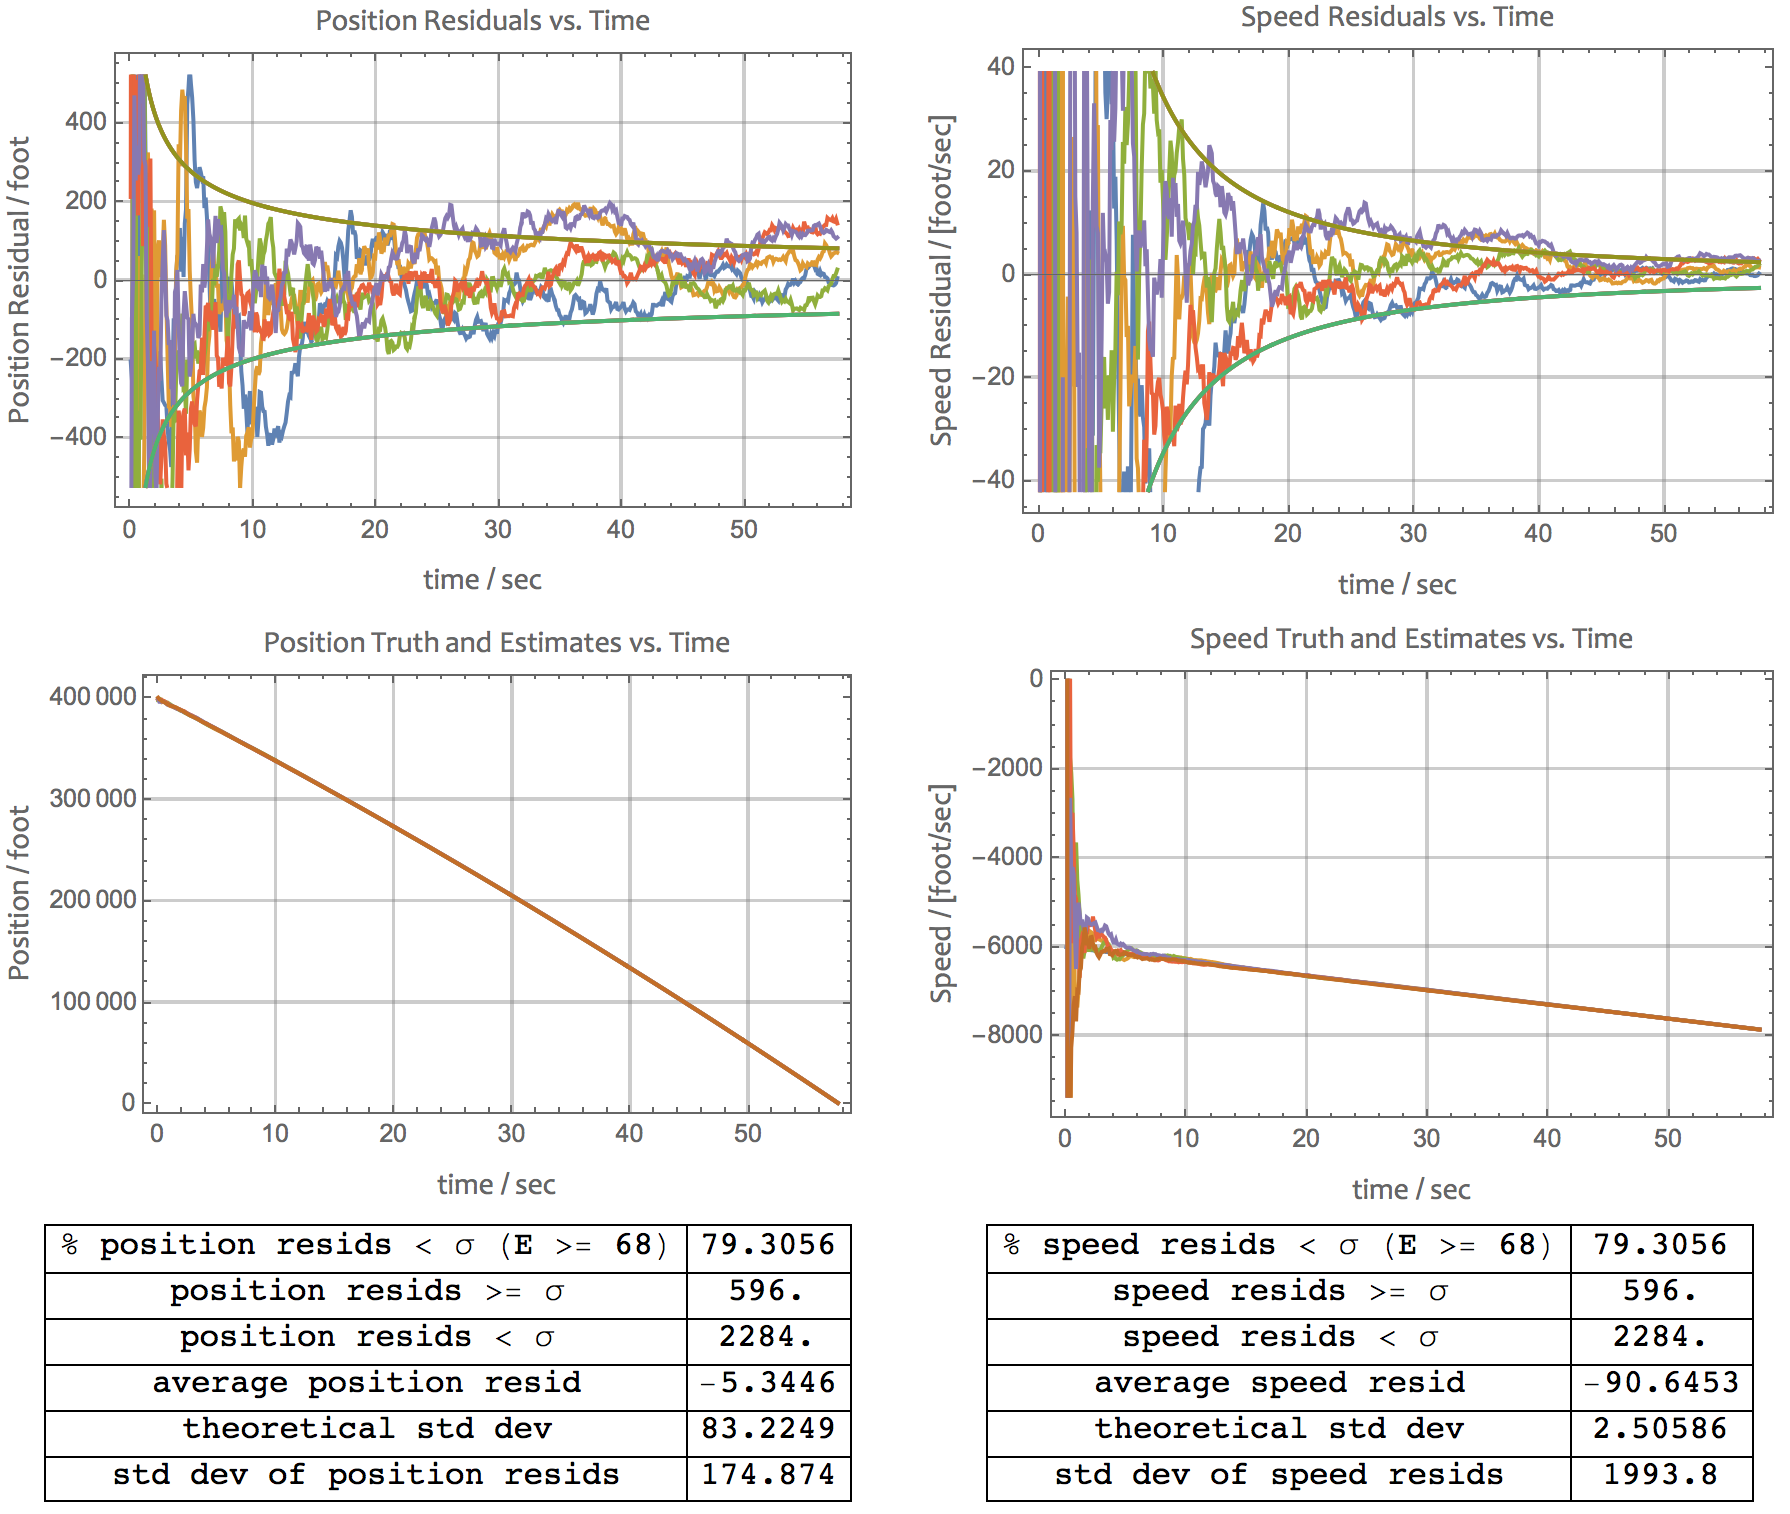
\includegraphics[width=.9\linewidth]{BigResults.png}
\caption{\label{fig:orgparagraph1}
Simulated tracking of a falling object}
\end{figure}

\noindent We test this filter over a sequence of fake
observations tracking an object from an initial height of \(400,000\,\textrm{ft}\)
and initial speed of \(-6,000\,\textrm{ft}/\textrm{s}\) and from time \(t=\si{0}{s}\)
to \(t=57.5\) sec, just before impact at \(h=0\,\textrm{ft}\). We take one
observation every tenth of a second, so \(\delta t={0.10}\,\textrm{s}\). We compare the
two states \(h(t)\) and \(\dot{h}(t)\) with ground truth and their residuals with
the theoretical sum of squared residuals in the matrix \(\mathbold{P}\). The
results are shown in figure \ref{fig:orgparagraph1}, showing good statistics over five
consecutive runs and qualitatively matching the results in the reference.

The ground truth is

\begin{equation*}
h(t) = h_0 + {\dot{h}}_0\,t + g\,t^2/2
\end{equation*}

\noindent where

\begin{equation*}
\begin{matrix}
h_0 = 400,000\,\textrm{ft}, & {\dot{h}}_0 = -6,000\,\textrm{ft}/\textrm{sec}
\end{matrix}
\end{equation*}

\noindent and we generate fake noisy observations by sampling a Gaussian
distribution of zero mean and standard deviation \(1,000\,\textrm{ft}\). We do not
need process noise for this example. It's often added during debugging of a
Kalman filter to compensate for underfitting or overfitting an inappropriate
model. It's also appropriate when we know that the process is stochastic or
noisy and have an estimate of its covariance.

\section{Concluding Remarks}
\label{sec:orgheadline8}

It's easy to add system dynamics to a static Kalman filter. Expressed as the
accumulator function for a fold, the filter is decoupled from the environment in
which it runs. We can run exactly the same code, even and especially the same
binary, over arrays in memory, lazy streams, asynchronous observables, any data
source that can support a \emph{fold} operator. Such flexibility of deployment allows
us to address the difficult issues of modeling, statistics, and numerics in
friendly environments where we have large memories and powerful debugging tools,
then to deploy with confidence in unfriendly, real-world environments where we
have small memories, asynchronous, real-time data delivery, and seldom more than
logging for forensics.
Emacs 24.5.1 (Org mode 8.3.4)
\end{document}